\section{Versuchsaufbau/-durchführung}

\subsection{Bestimmung der Durchlasskurve für den $LC$- und $LC_1 C_2$ Kette}
Zunächst wird der Aufbau, wie in Abbildung \ref{fig:aufbau_durchlass} zusehen aufgebaut.
\begin{figure}
  \centering
  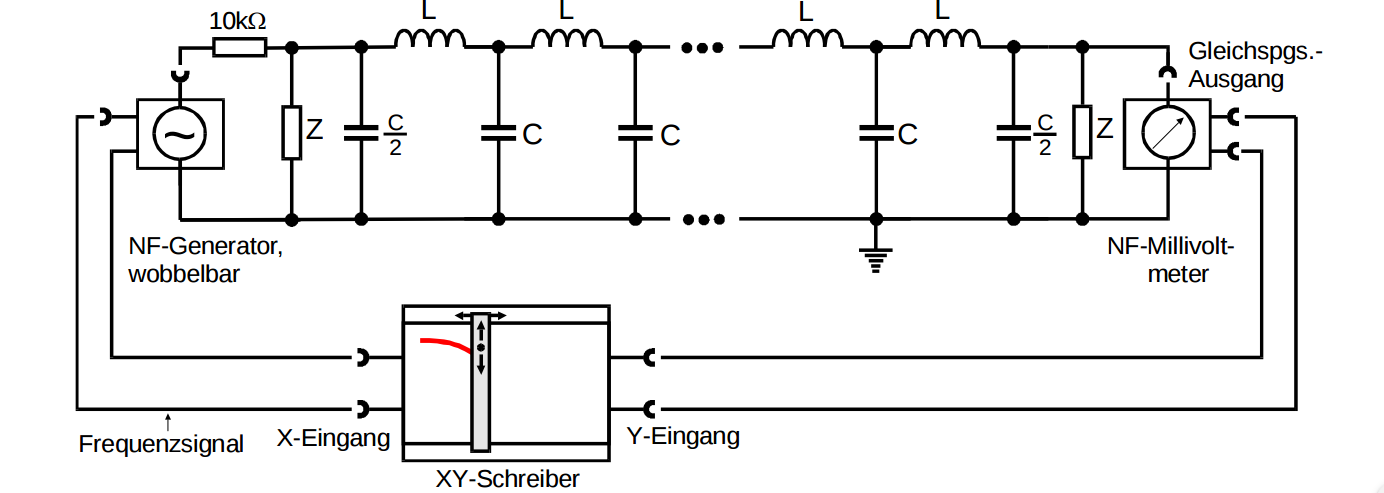
\includegraphics[width=0.8\textwidth]{bilder/versuchsaufbau_1.png}
  \caption{Versuchsaufbau für die bestimmung der Durchlasskurve}
  \label{fig:aufbau_durchlass}
\end{figure}

Bei dem NF-Generator wird ein Frequenz Sweep eingestellt.7
Am Kettenanfang und -ende werden die Wiederstände $Z$ auf den theoretisch 
berechnetetn Wellenwiederstand eingestellt.
In dem Frequenzbereich des Sweeps muss die Grenzfrequenzen liegen, bei der die 
Kettenschaltung Strom undurchlässig wird.
Die am Kettenende anliegende Spannung und die vom Generator ausgegebenen Frequenzen, 
werden an einem XY-Schreiber gegen einander aufgetragen.
Wichtig dabei ist, das bei beliebigen Punkten auf dem vom XY-Schreiber
erzeugten Plot, die gerade anliegende Frequenz bekannt ist. %Hier noch mehr dazu ?


\subsection{Bestimmung der Dispersionskurve}
Der Versuch wird wie in Abbildung \ref{fig:aufbau_dispersion} zusehen ist, aufgebaut.
\begin{figure}
  \centering
  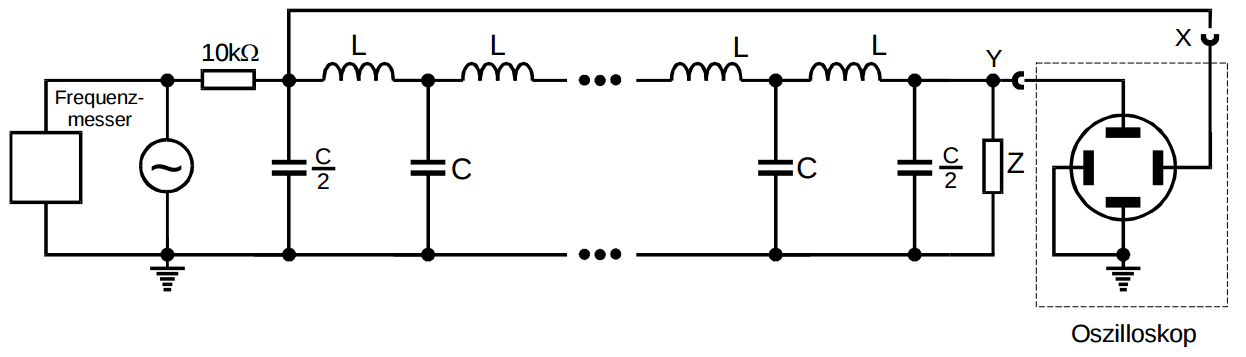
\includegraphics[width=0.8\textwidth]{bilder/versuchsaufbau_dispersion.png}
  \caption{Versuchsaufbau für die Messung der Dispersionskurve}
  \label{fig:aufbau_dispersion}
\end{figure}

Anschließend werden für die verwendeten $L$, $C_1$ und $C_2$ die Wellenwiederstände berechnet
und die An- und Abschlusswiederstände $Z$ auf diesen Wert eingestellt.
Mithilfe von Lissajou-Figuren werden nun die Frequezen bestmmt, wo eine Phasenverschiebung von $\pi$ 
vorhanden ist. Anschließend kann dann mit der Anzahl der Kettenglieder auf die, 
Phasenverschiebung pro Kettengleid geschlossen werden.

\subsection{Ausmessung der stehende Welle}
Der Versuch wird nach Abb. \ref{fig:aufbau_dispersion} aufgebaut.
Nun wird einmal mit und einmal ohne Wellenwiederstand $Z$, die Spannung einem Millivoltmeter gemessen.
Zunächst wird die Spannung am Kettenanfang abgegriffen, um so ein frequenzabhängiges Spannungsmaximum 
zufinden. Für die ersten beiden Maxima, werden bei allen Kettengliedern die anliegendes Spannung gemessen.
Für die restlichen Maxima werden nur die dazugehörigen Frequenzen notiert.
